%%%%%%%%%%%%%%%%%%%%%%%%%%%%%%%%%%%%%%%%%
% Beamer Presentation
% LaTeX Template
% Version 1.0 (10/11/12)
%
% This template has been downloaded from:
% http://www.LaTeXTemplates.com
%
% License:
% CC BY-NC-SA 3.0 (http://creativecommons.org/licenses/by-nc-sa/3.0/)
%
%%%%%%%%%%%%%%%%%%%%%%%%%%%%%%%%%%%%%%%%%

%----------------------------------------------------------------------------------------
%	PACKAGES AND THEMES
%----------------------------------------------------------------------------------------

\documentclass[UTF8,aspectratio=169,14pt]{ctexbeamer}

\usepackage{hyperref}
\hypersetup{
	colorlinks=true,
	linkcolor=red,
	anchorcolor=blue,
	citecolor=green
}

\mode<presentation> {
	
	% The Beamer class comes with a number of default slide themes
	% which change the colors and layouts of slides. Below this is a list
	% of all the themes, uncomment each in turn to see what they look like.
	
	%\usetheme{default}
	%\usetheme{AnnArbor}
	%\usetheme{Antibes}
	%\usetheme{Bergen}
	%\usetheme{Berkeley}
	%\usetheme{Berlin}
	%\usetheme{Boadilla}
	%\usetheme{CambridgeUS}
	%\usetheme{Copenhagen}
	%\usetheme{Darmstadt}
	%\usetheme{Dresden}
	%\usetheme{Frankfurt}
	%\usetheme{Goettingen}
	%\usetheme{Hannover}
	%\usetheme{Ilmenau}
	%\usetheme{JuanLesPins}
	%\usetheme{Luebeck}
	\usetheme{Madrid}
	%\usetheme{Malmoe}
	%\usetheme{Marburg}
	%\usetheme{Montpellier}
	%\usetheme{PaloAlto}
	%\usetheme{Pittsburgh}
	%\usetheme{Rochester}
	%\usetheme{Singapore}
	%\usetheme{Szeged}
	%\usetheme{Warsaw}
	
	% As well as themes, the Beamer class has a number of color themes
	% for any slide theme. Uncomment each of these in turn to see how it
	% changes the colors of your current slide theme.
	
	%\usecolortheme{albatross}
	%\usecolortheme{beaver}
	%\usecolortheme{beetle}
	%\usecolortheme{crane}
	%\usecolortheme{dolphin}
	%\usecolortheme{dove}
	%\usecolortheme{fly}
	%\usecolortheme{lily}
	%\usecolortheme{orchid}
	%\usecolortheme{rose}
	%\usecolortheme{seagull}
	%\usecolortheme{seahorse}
	%\usecolortheme{whale}
	%\usecolortheme{wolverine}
	
	%\setbeamertemplate{footline} % To remove the footer line in all slides uncomment this line
	%\setbeamertemplate{footline}[page number] % To replace the footer line in all slides with a simple slide count uncomment this line
	
	%\setbeamertemplate{navigation symbols}{} % To remove the navigation symbols from the bottom of all slides uncomment this line
}

\usepackage{graphicx} % Allows including images
\graphicspath{{./figs/}}
\usepackage{booktabs} % Allows the use of \toprule, \midrule and \bottomrule in tables
\usepackage{longtable}
\usepackage{listings}
\usepackage{xcolor}
\lstset{numbers=left, %设置行号位置
	numberstyle=\tiny, %设置行号大小
	keywordstyle=\color{blue}, %设置关键字颜色
	commentstyle=\color[cmyk]{1,0,1,0}, %设置注释颜色
	frame=single, %设置边框格式
	escapeinside=``, %逃逸字符(1左面的键),用于显示中文
	%breaklines, %自动折行
	extendedchars=false, %解决代码跨页时,章节标题,页眉等汉字不显示的问题
	xleftmargin=2em,xrightmargin=2em, aboveskip=1em, %设置边距
	tabsize=4, %设置tab空格数
	showspaces=false %不显示空格
}
% Fonts
% \usepackage{libertine}
% \setmonofont{Courier}
\setCJKsansfont[ItalicFont=Noto Serif CJK SC Black, BoldFont=Noto Sans CJK SC Black]{Noto Sans CJK SC}


%----------------------------------------------------------------------------------------
% TITLE PAGE
%----------------------------------------------------------------------------------------

\title[第20讲]{第二十讲 :I/O子系统} % The short title appears at the bottom of every slide, the full title is only on the title page
\subtitle{第1节:设备接口}
\author{向勇、陈渝、李国良} % Your name
\institute[清华大学] % Your institution as it will appear on the bottom of every slide, may be shorthand to save space
{
  清华大学计算机系 \\ % Your institution for the title page
  \medskip
  \textit{xyong,yuchen@tsinghua.edu.cn} % Your email address
}
\date{\today} % Date, can be changed to a custom date

\begin{document}

\begin{frame}
\titlepage % Print the title page as the first slide
\end{frame}

%----------------------------------------------
\begin{frame}
\frametitle{提纲} % Table of contents slide, comment this block out to remove it
\tableofcontents % Throughout your presentation, if you choose to use \section{} and \subsection{} commands, these will automatically be printed on this slide as an overview of your presentation

%% itemize
%Ref:
%    \begin{itemize}
%        \item \href{http://osq.cs.berkeley.edu/public/JFoster-Drivers.ppt}{Linux Device Drivers Overview}
%        \item \href{http://ermak.cs.nstu.ru/understanding.linux.kernel.pdf}{Understanding the Linux Kernel}
%    \end{itemize}

\end{frame}
%----------------------------------------------
%%  PRESENTATION SLIDES
%----------------------------------------------
\section{第1节:设备接口} % Sections can be created in order to organize your presentation into discrete blocks, all sections and subsections are automatically printed in the table of contents as an overview of the talk
%----------------------------------------------
\subsection{常见设备接口类型} % A subsection can be created just before a set of slides with a common theme to further break down your presentation into chunks
%----------------------------------------------
\begin{frame}[fragile]
    \frametitle{I/O子系统}
    %    \framesubtitle{xxxx}
    要解决什么问题?
    \begin{itemize}
        \item 为何设备的差异性那么大?
        \item 为何要管理设备? \pause
        \item 如何统一对设备的访问接口?
        \item 为何要对设备建立抽象? \pause
        \item 如何感知设备的状态并管理设备?
        \item 如何提高CPU与设备的访问性能?
        \item 如果保证I/O操作的可靠性?
    \end{itemize}
    %    \begin{figure}
    %        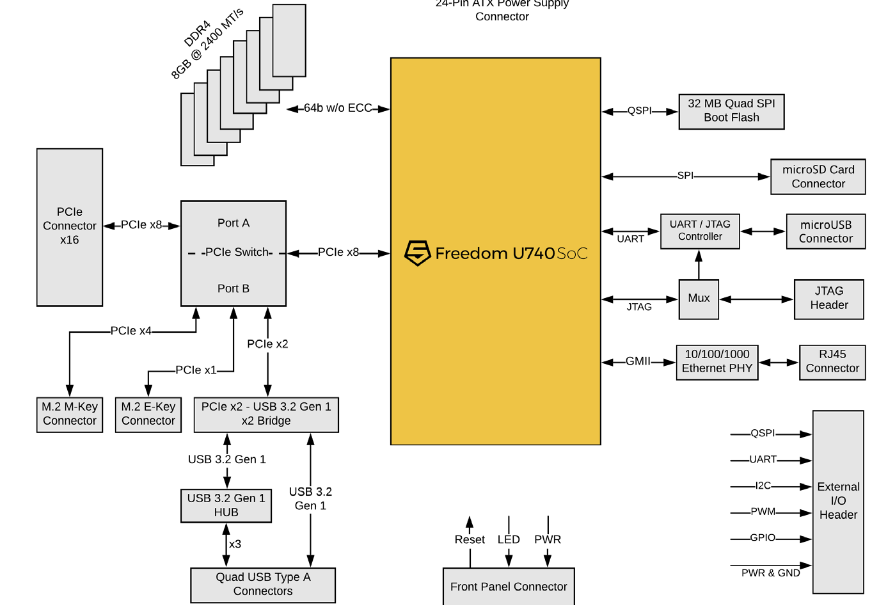
\includegraphics[width=0.3\linewidth]{figs/u740-arch.png}
    %        %  \caption{xxxx}
    %    \end{figure}
\end{frame}
%----------------------------------------------
\begin{frame}[fragile]
    \frametitle{常见设备接口类型}
    %    \framesubtitle{xxxx}
    设备的发展
    \begin{itemize}
        \item 简单设备:CPU可通过I/O接口直接控制I/O设备
        \item 多设备:CPU与I/O设备之间增加了一层I/O控制器和总线BUS
        \item 支持中断的设备:提高CPU利用率
        \item 高吞吐量设备:支持DMA
        \item 各种其他设备:GPU、声卡、智能网卡、RDMA
        \item 连接方式:直连、(设备/中断)控制器、总线、分布式
    \end{itemize}
    %    \begin{figure}
    %        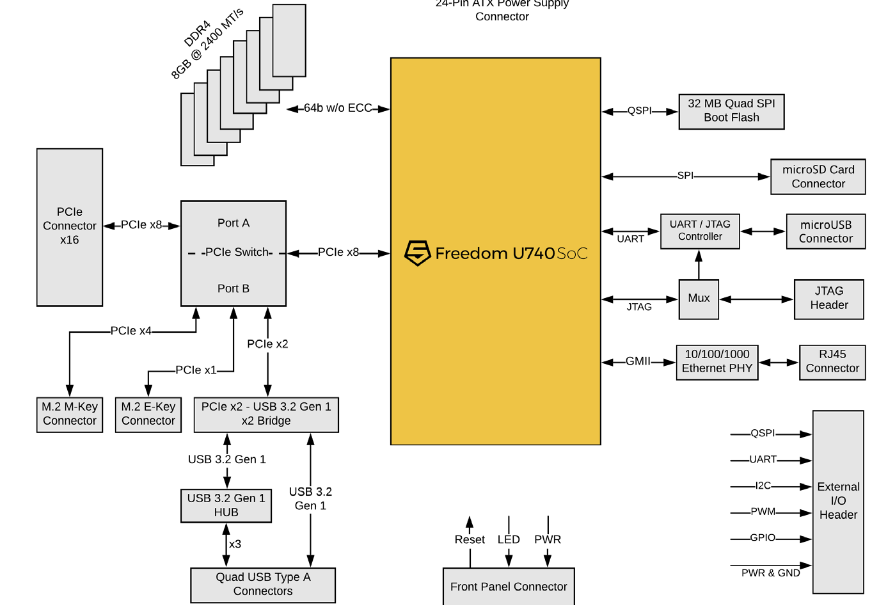
\includegraphics[width=0.3\linewidth]{figs/u740-arch.png}
    %        %  \caption{xxxx}
    %    \end{figure}
\end{frame}
%----------------------------------------------
\begin{frame}[fragile]
    \frametitle{常见设备接口类型}
%    \framesubtitle{xxxx}
    \begin{itemize}
    \item 字符设备
    \item 块设备
    \item 网络设备
    \end{itemize}
    \begin{figure}
    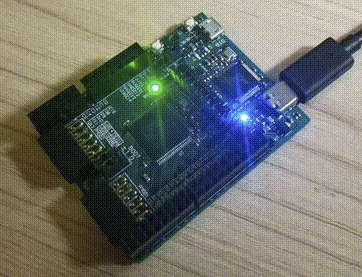
\includegraphics[width=0.4\linewidth]{figs/embed-dev.png}
    \caption{RISC-V嵌入式开发板}
\end{figure}
\end{frame}
%----------------------------------------------
% #### Linux I/O Architecture
% 
% ##### Linux I/O Architecture
% 
% ![io-architecture](figs/io-architecture.png)
% 

%----------------------------------------------
\begin{frame}[fragile]
    \frametitle{常见设备接口类型}
    %    \framesubtitle{xxxx}
    字符设备
    \begin{itemize}
        \item 如: GPIO, 键盘/鼠标, 串口等
    \end{itemize}
    \begin{figure}
        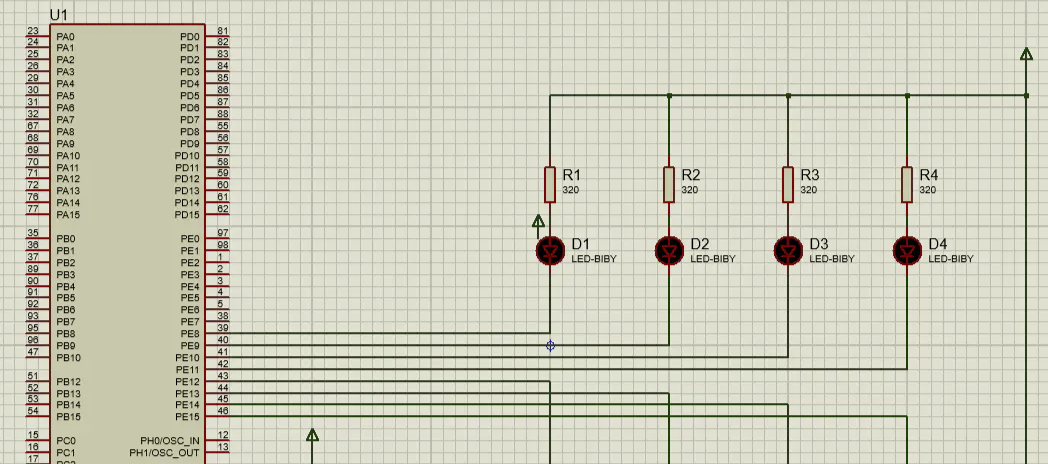
\includegraphics[width=0.75\linewidth]{figs/char-led.png}
          \caption{GPIO LED light}
    \end{figure}
\end{frame}

%----------------------------------------------
\begin{frame}[fragile]
    \frametitle{常见设备接口类型}
    %    \framesubtitle{xxxx}
    字符设备
    \begin{itemize}
        % General Purpose Input/Output --GPIO
        \item 如: GPIO, \emph{键盘}/鼠标, 串口等
    \end{itemize}
    \begin{figure}
        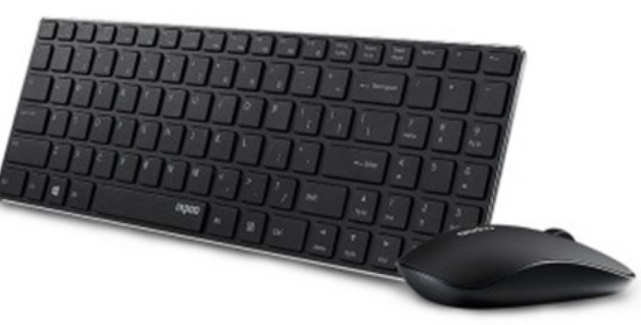
\includegraphics[width=0.47\linewidth]{figs/char-dev.png}
        \caption{键盘}
    \end{figure}
\end{frame}
%----------------------------------------------
\begin{frame}[fragile]
    \frametitle{常见设备接口类型}
    %    \framesubtitle{xxxx}
    字符设备
    \begin{itemize}
        \item 如: GPIO, \emph{键盘}/鼠标, 串口等
    \end{itemize}
    \begin{figure}
        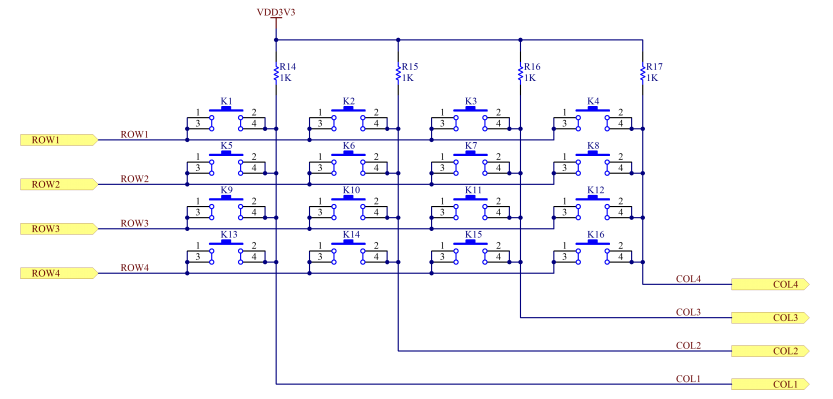
\includegraphics[width=0.6\linewidth]{figs/char-keyboard.png}
        \caption{键盘电路}
    \end{figure}
\end{frame}

%----------------------------------------------
\begin{frame}[fragile]
    \frametitle{常见设备接口类型}
    %    \framesubtitle{xxxx}
    字符设备
    \begin{itemize}
        \item 如: GPIO, \emph{键盘}/鼠标, 串口等
    \end{itemize}
    \begin{figure}
        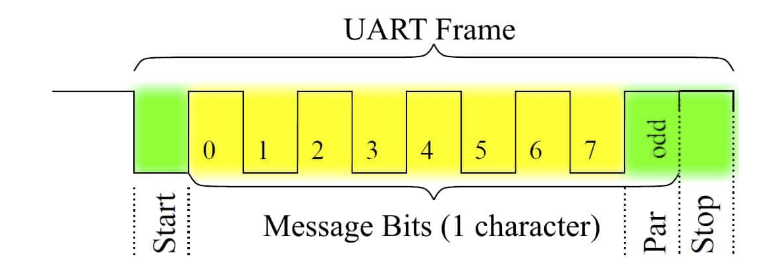
\includegraphics[width=0.6\linewidth]{figs/char-uart.png}
        \caption{UART串口通信}
    \end{figure}
\end{frame}
%----------------------------------------------
% ##### Block Driver
% 
% ![block-driver](figs/block-driver.png)
% 
%----------------------------------------------
\begin{frame}[fragile]
    \frametitle{常见设备接口类型}
    %    \framesubtitle{xxxx}
    块设备
    \begin{itemize}
        \item 如: 磁盘驱动器、磁带驱动器、光驱等
    \end{itemize}
    \begin{figure}
        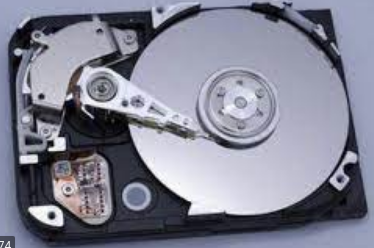
\includegraphics[width=0.47\linewidth]{figs/blk-dev.png}
        %  \caption{xxxx}
    \end{figure}
\end{frame}
%----------------------------------------------
% ##### Network Driver
% 
% ![network-driver](figs/network-driver.png)
\begin{frame}[fragile]
    \frametitle{常见设备接口类型}
    %    \framesubtitle{xxxx}
    网络设备
    \begin{itemize}
        \item 如: ethernet、wifi、bluetooth等
    \end{itemize}
    \begin{figure}
        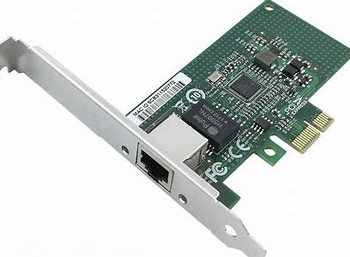
\includegraphics[width=0.47\linewidth]{figs/net-dev.png}
        %  \caption{xxxx}
    \end{figure}
\end{frame}
%----------------------------------------------
\begin{frame}
\frametitle{提纲} % Table of contents slide, comment this block out to remove it
\tableofcontents % Throughout your presentation, if you choose to use \section{} and \subsection{} commands, these will automatically be printed on this slide as an overview of your presentation

%% itemize
%Ref:
%    \begin{itemize}
%        \item \href{http://osq.cs.berkeley.edu/public/JFoster-Drivers.ppt}{Linux Device Drivers Overview}
%        \item \href{http://ermak.cs.nstu.ru/understanding.linux.kernel.pdf}{Understanding the Linux Kernel}
%    \end{itemize}

\end{frame}
%----------------------------------------------
\subsection{设备访问特征} % A subsection can be created just before a set of slides with a common theme to further break down your presentation into chunks
%----------------------------------------------
\begin{frame}[fragile]
    \frametitle{设备访问特征}
%    \framesubtitle{xxxx}
    字符设备
    \begin{itemize}
        \item 以字节为单位顺序访问
        \item I/O命令:get()、put()等
        \item 通常使用文件访问接口和语义
    \end{itemize}
    \begin{figure}
    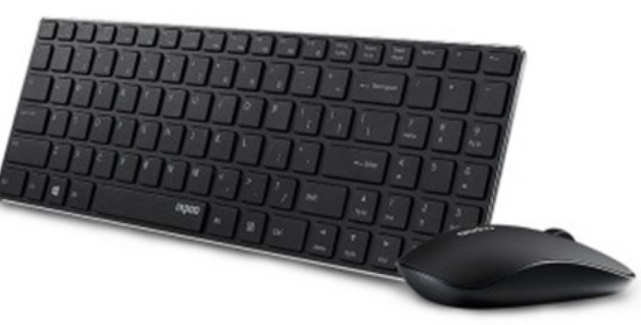
\includegraphics[width=0.4\linewidth]{figs/char-dev.png}
  %  \caption{xxxx}
    \end{figure}
\end{frame}
%----------------------------------------------
% #### Device Driver
% 
\begin{frame}[fragile]
    \frametitle{设备访问特征}
    %    \framesubtitle{xxxx}
    块设备
    \begin{itemize}
        \item 均匀的数据块访问
        \item I/O命令:原始I/O或文件系统接口、内存映射文件访问
        \item 通常使用文件访问接口和语义
    \end{itemize}
    \begin{figure}
        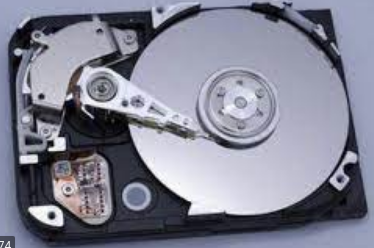
\includegraphics[width=0.3\linewidth]{figs/blk-dev.png}
        %  \caption{xxxx}
    \end{figure}
\end{frame}
%----------------------------------------------
% #### Device Driver
% 
\begin{frame}[fragile]
    \frametitle{设备访问特征}
    %    \framesubtitle{xxxx}
    网络设备
    \begin{itemize}
        \item 格式化报文交换
        \item I/O命令:send/receive 网络报文, 通过网络接口支持多种网络协议
        \item 通常使用socket访问接口和语义
    \end{itemize}
    \begin{figure}
        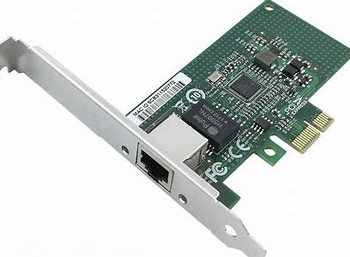
\includegraphics[width=0.3\linewidth]{figs/net-dev.png}
        %  \caption{xxxx}
    \end{figure}
\end{frame}

%----------------------------------------------
\begin{frame}[fragile]
    \frametitle{设备访问特征:RISC-V PC的外设}
    %    \framesubtitle{xxxx}
%    设备的发展
%    \begin{itemize}
%        \item 简单设备:CPU可通过I/O接口直接控制I/O设备
%        \item 多设备:CPU与I/O设备之间增加了一层I/O控制器和总线BUS
%        \item 支持中断的设备:提高CPU利用率
%        \item 高吞吐量设备:支持DMA
%    \end{itemize}
    \begin{figure}
        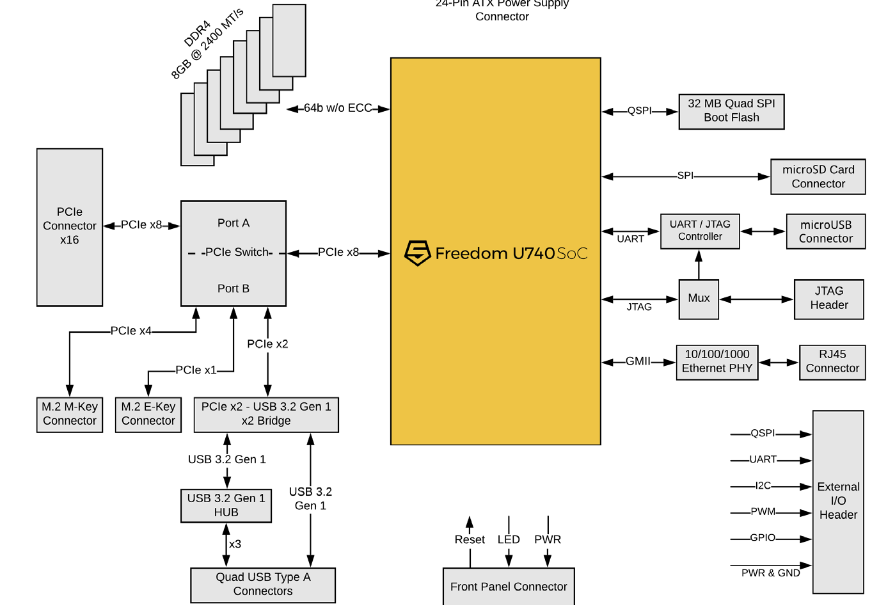
\includegraphics[width=0.65\linewidth]{figs/u740-arch.png}
        %  \caption{xxxx}
    \end{figure}
\end{frame}
%----------------------------------------------
\begin{frame}
\frametitle{提纲} % Table of contents slide, comment this block out to remove it
\tableofcontents % Throughout your presentation, if you choose to use \section{} and \subsection{} commands, these will automatically be printed on this slide as an overview of your presentation

%% itemize
%Ref:
%    \begin{itemize}
%        \item \href{http://osq.cs.berkeley.edu/public/JFoster-Drivers.ppt}{Linux Device Drivers Overview}
%        \item \href{http://ermak.cs.nstu.ru/understanding.linux.kernel.pdf}{Understanding the Linux Kernel}
%    \end{itemize}

\end{frame}
%----------------------------------------------
\subsection{设备传输方式} %
%----------------------------------------------
\begin{frame}[fragile]
    \frametitle{设备传输方式}
    %    \framesubtitle{xxxx}
        \begin{itemize}
            \item 程序控制I/O(PIO, Programmed I/O)
            \item Interrupt based I/O
            \item 直接内存访问(DMA)
        \end{itemize}
%    \begin{figure}
%        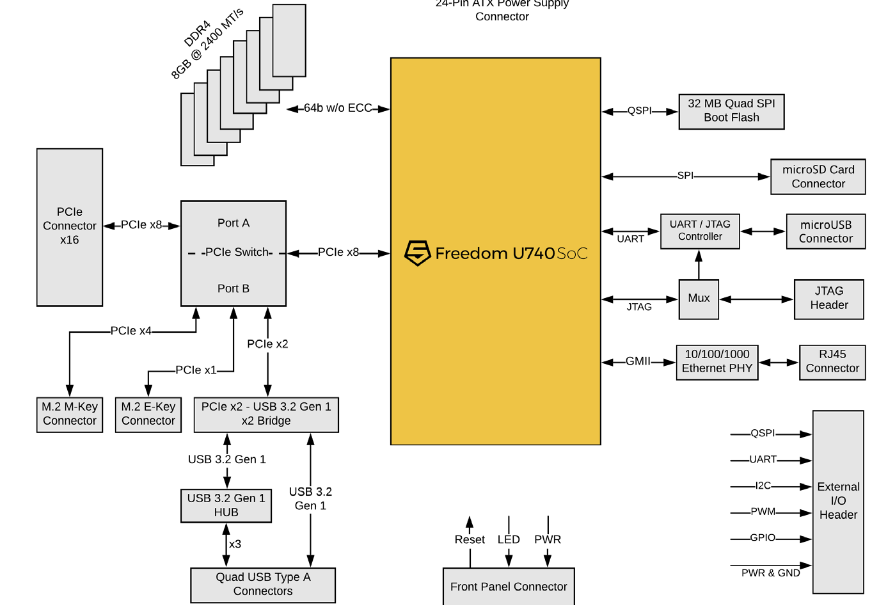
\includegraphics[width=1.\linewidth]{figs/u740-arch.png}
%        %  \caption{xxxx}
%    \end{figure}
\end{frame}
%----------------------------------------------
\begin{frame}[fragile]
    \frametitle{设备传输方式}
    %    \framesubtitle{xxxx}
    程序控制I/O(PIO, Programmed I/O)
    \begin{itemize}
        \item Port-mapped的PIO(PMIO):通过CPU的in/out指令
        \item Memory-mapped的PIO(MMIO):通过load/store传输所有数据
        \item 硬件简单,编程容易
        \item 消耗的CPU时间和数据量成正比
        \item 适用于简单的、小型的设备I/O
        \item I/O设备通知CPU:PIO方式的轮询
    \end{itemize}
    %    \begin{figure}
    %        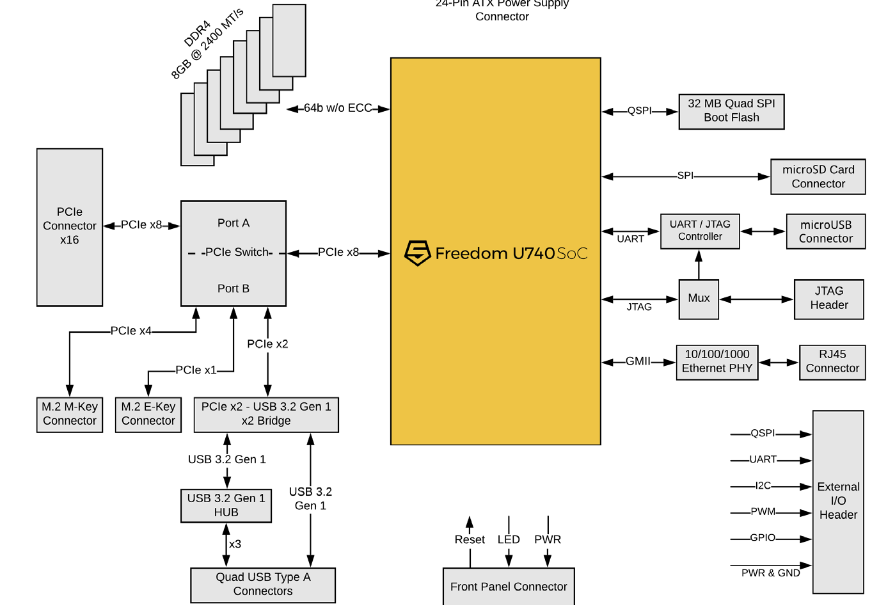
\includegraphics[width=1.\linewidth]{figs/u740-arch.png}
    %        %  \caption{xxxx}
    %    \end{figure}
\end{frame}
%----------------------------------------------
\begin{frame}[fragile]
    \frametitle{中断传输方式}
    %    \framesubtitle{xxxx}
    中断传输方式
    \begin{itemize}
        \item I/O设备向CPU发送中断请求信号:将数据准备好等状态信息通知CPU
        \item 支持中断的设备类型和中断类型逐步增加
        \item 需要同时设置CPU和中断控制器
        \item 编程比较麻烦
        \item CPU利用率高
        \item 适用于比较复杂的I/O设备
        \item I/O设备通知CPU:中断方式的提醒
    \end{itemize}
    %    \begin{figure}
    %        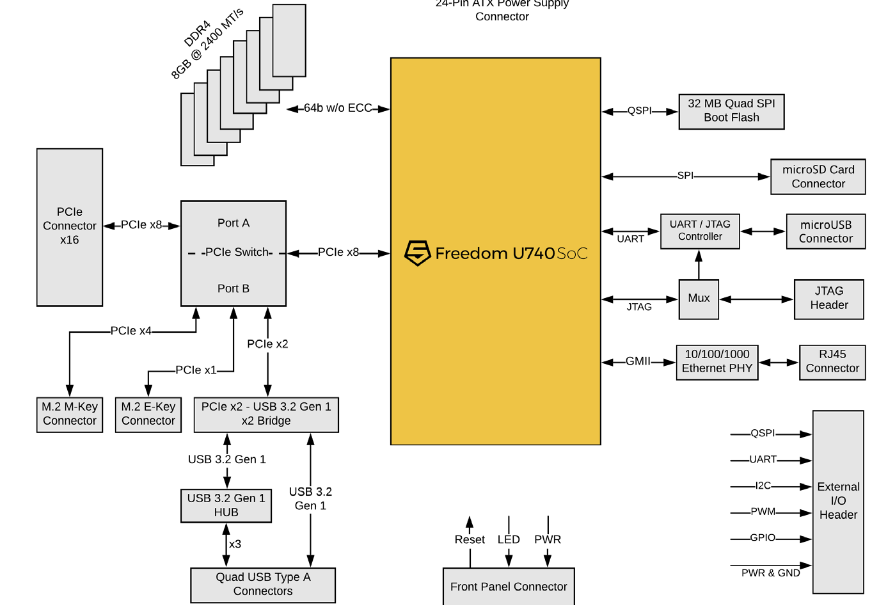
\includegraphics[width=1.\linewidth]{figs/u740-arch.png}
    %        %  \caption{xxxx}
    %    \end{figure}
\end{frame}

%----------------------------------------------
\begin{frame}[fragile]
    \frametitle{中断传输方式}
    %    \framesubtitle{xxxx}
%    中断传输方式
%    \begin{itemize}
%        \item I/O设备想通知CPU或有了CPU需要的数据,便会发出中断请求信号
%        \item 可中断的设备和中断类型逐步增加
%        \item 除了需要设置CPU,还需设置中断控制器
%        \item 编程比较麻烦
%        \item CPU利用率高
%        \item 适用于比较复杂的I/O设备
%        \item I/O设备通知CPU:中断方式的提醒
%    \end{itemize}
        \begin{figure}
            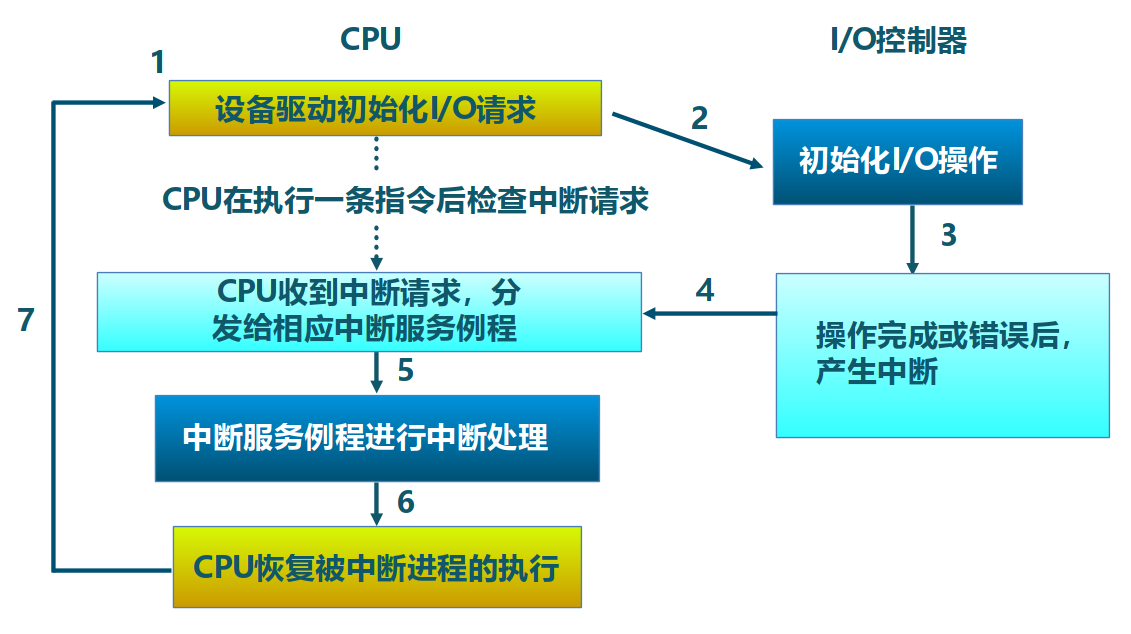
\includegraphics[width=0.8\linewidth]{figs/interrupt-steps.png}
            %  \caption{xxxx}
        \end{figure}
\end{frame}
%----------------------------------------------
\begin{frame}[fragile]
    \frametitle{DMA传输方式}
    %    \framesubtitle{xxxx}
    中断传输方式
    \begin{itemize}
        \item 设备控制器可直接访问系统总线
        \item 控制器直接与内存互相传输数据
        \item 需要同时设置CPU、DMA控制器和中断控制器
        \item 编程比较麻烦,需要CPU参与设置
        \item 设备传输数据不影响CPU
        \item 适用于高吞吐量I/O设备
    \end{itemize}
    %    \begin{figure}
    %        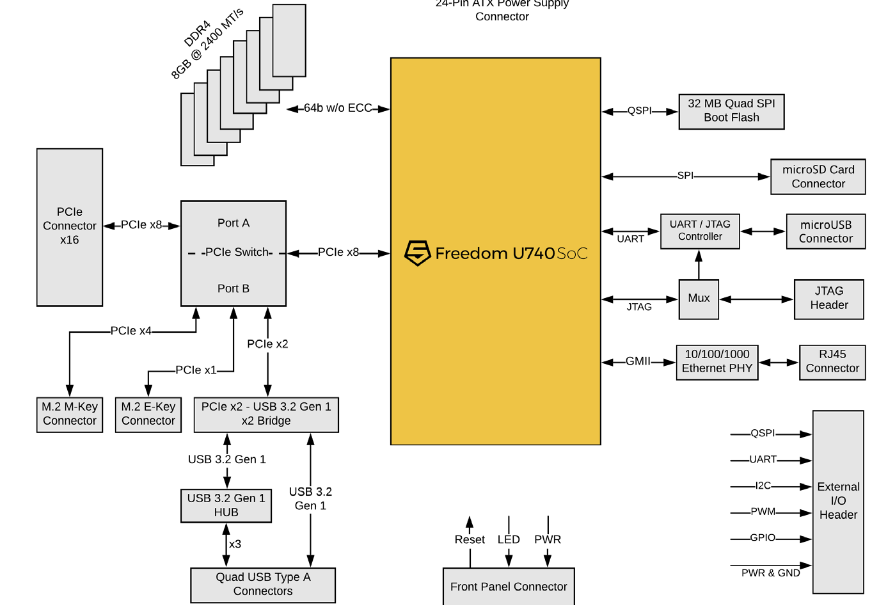
\includegraphics[width=1.\linewidth]{figs/u740-arch.png}
    %        %  \caption{xxxx}
    %    \end{figure}
\end{frame}
%----------------------------------------------
\begin{frame}[fragile]
    \frametitle{CPU与设备的连接}
    %    \framesubtitle{xxxx}
    %    中断传输方式
    %    \begin{itemize}
    %        \item 设备控制器可直接访问系统总线
    %        \item 控制器直接与内存互相传输数据
    %        \item 除了需要设置CPU,还需设置中断控制器
    %        \item 编程比较麻烦,需要CPU参与设置
    %        \item 设备传输数据不影响CPU
    %        \item 适用于高吞吐量I/O设备
    %    \end{itemize}
    \begin{figure}
        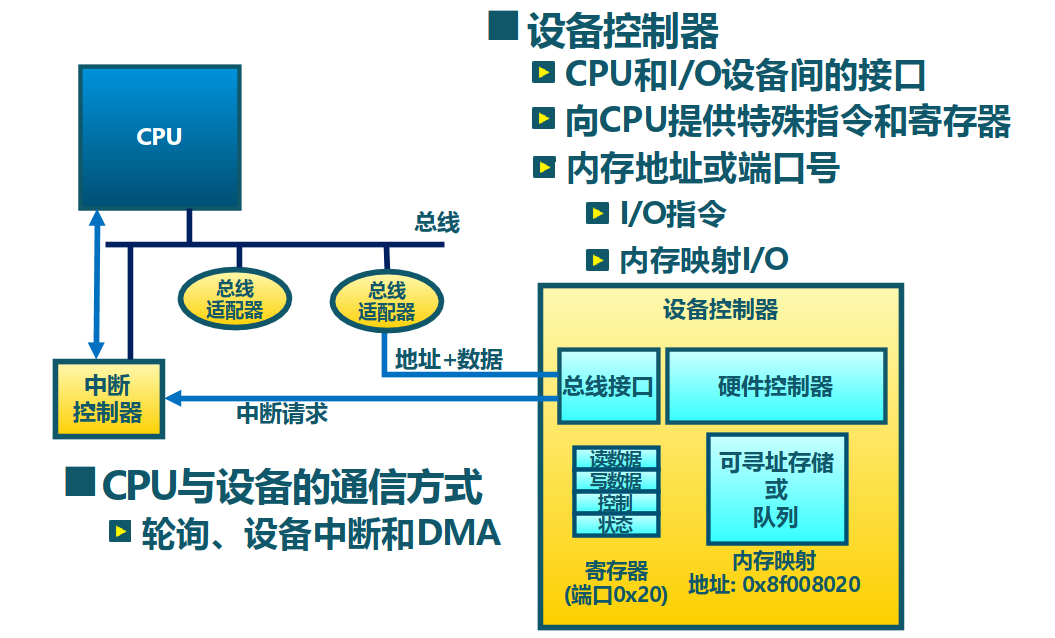
\includegraphics[width=0.8\linewidth]{figs/cpu-connect-dev.png}
        %  \caption{xxxx}
    \end{figure}
\end{frame}
%----------------------------------------------
\begin{frame}[fragile]
    \frametitle{读取磁盘数据的例子}
    %    \framesubtitle{xxxx}
%    中断传输方式
%    \begin{itemize}
%        \item 设备控制器可直接访问系统总线
%        \item 控制器直接与内存互相传输数据
%        \item 除了需要设置CPU,还需设置中断控制器
%        \item 编程比较麻烦,需要CPU参与设置
%        \item 设备传输数据不影响CPU
%        \item 适用于高吞吐量I/O设备
%    \end{itemize}
        \begin{figure}
            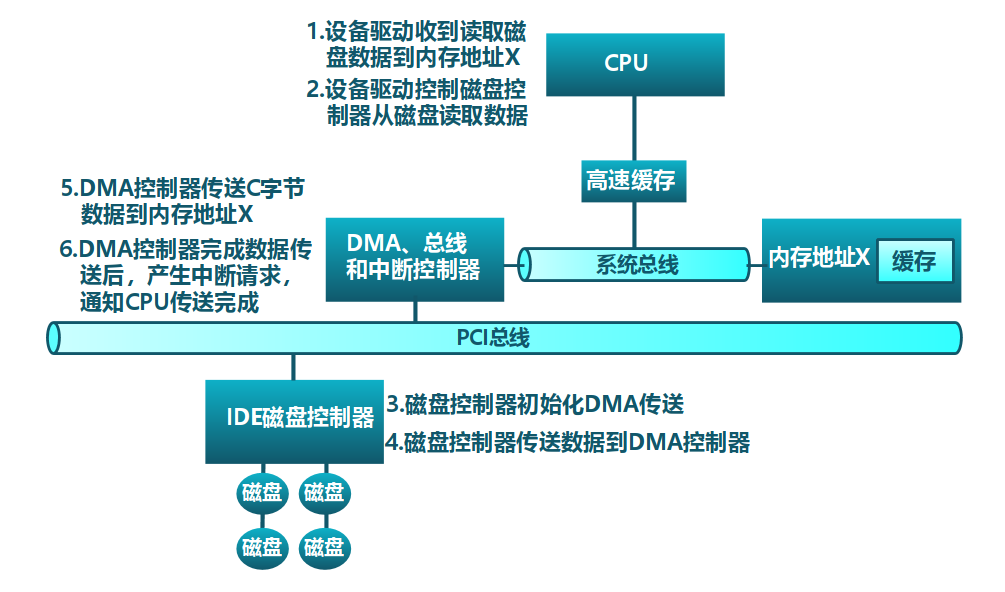
\includegraphics[width=0.8\linewidth]{figs/access-disk-io.png}
            %  \caption{xxxx}
        \end{figure}
\end{frame}
%----------------------------------------------

\end{document}
